\subsection{Team Organization}

At the beginning of the project, it was decided that the group would split into 3 different teams to allow people to work on the sections they were interested in.
These 3 teams were based around, the ESP-32, the Raspberry Pi and the website as seen in figure \ref{fig:grouporg}.

\begin{figure}[H]        
    \centering
    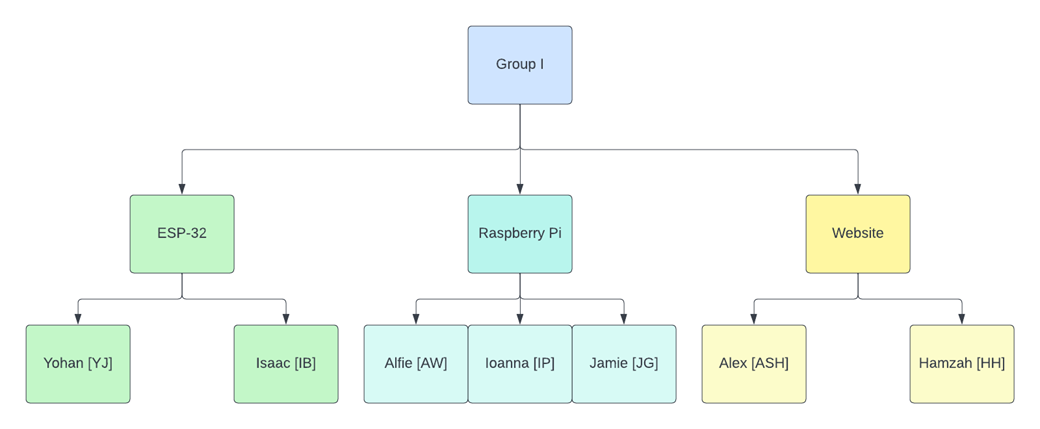
\includegraphics[width=.66\textwidth]{Chapter 6/Reflection/GroupDiagram.png}
    \caption{Group Organization Diagram}
    \label{fig:grouporg}
\end{figure} 

Unfortunately, due to issues that are explained in chapters 3, 4 and 5,
we were not able to fully adhered to the plan meaning that group members had to start working outside of these predefined groups.
This led to rapid changes in the project without researching the substitute methods.

To add, the following Gantt Chart in figure \ref{fig:gantt} was produced.

\begin{figure}[H]        
    \centering
    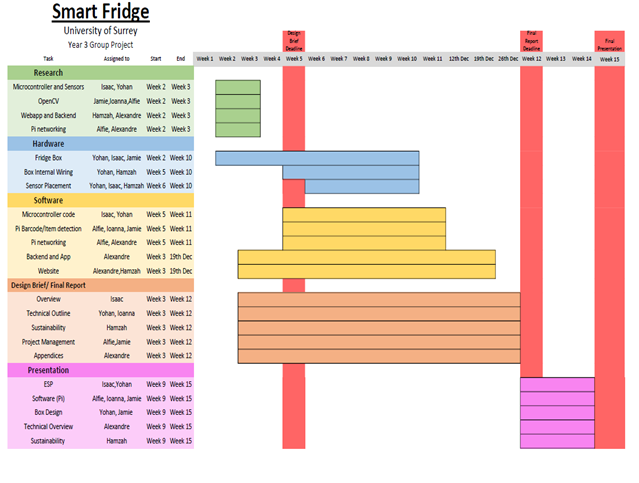
\includegraphics[width=1\textwidth]{Chapter 6/Reflection/GanttChart.png}
    \caption{Gantt Planning Chart}
    \label{fig:gantt}
\end{figure} 

\subsection{Isaac Baglin [IB]}
My goal for this project was to develop skills in systems engineering.
To do this, I put myself on the microprocessor team so that I could plan, design, and integrate subsystems.
During the earlier weeks of the project, I helped plan the project by breaking the overall task into smaller subsystems.
It was also important that we discussed the dependencies between sections to make integration easier.
It was my personal responsibility to test the weight sensor, the buzzer and the esp32 camera module.
Within these tasks I selected the components, programmed them, and integrated them into the larger system.
This meant I was able to contribute both to hardware and software elements of the project.

The largest challenge that I faced was that the esp32 camera module didn't have a higher enough resolution to pick up barcodes in images.
This camera module was designed to take videos not isolated images therefore programming the module to take individual images was very challenging and time consuming.
Given the issue was a resolution problem, I had no choice but to scrap the module.
Thankfully, because of the planning in the earlier weeks of the project, we had a web camera available which could be used instead.
In future projects, more time should be taken to research the components and their feasibility.
The esp32 camera was chosen because it was pre-built on the microprocessor however because it wasn't designed to take individual images, the module shouldn't have been pursued to start with.
The time wasted on this module could have been spent adding additional features to the product or further assisting other group members with their sections.

Despite this one issue I feel as though I contributed greatly to the group's workload, I also acted as a valuable group member by being a key planner for the project by constantly contributing to the group discussions.
Given how dependent other subsystems were on the hardware, I made sure to meet all my personal deadlines as early as possible.
I was able to meet my personal objects of planning, designing, and integrating subsystems and the problems with the camera module allowed me to learn the importance of feasibility reviews for future projects.

\subsection{Jamie Gomez [JG]}
Going into this project there were several goals I set for myself.
Among these were to develop my teamwork skills and to build on my knowledge from previous projects, possibly working in areas in which I have not worked before.
Within the first few weeks of the project, I was assigned to work on the OpenCV side of this project and I later contributed to the design of the box with CAD designs.

Within the OpenCV team, I specifically worked on barcode detection.
This involved researching various different methods of carrying out barcode detection using OpenCV, as well as testing them to choose the one that best fit the group's aims for this project.
Whist this part of the project contained relatively little teamwork at first, I felt that I worked towards this goal later on in the project when this needed to be integrated with the other OpenCV sections.

Despite having used CAD software such as SketchUp in the past, I had never had to work to such precise measurements and requirements.
Therefore, apart from finding solutions to the different design problems that arose, I was also forced to use this software differently to how I had done so in the past.
Therefore, I feel that this satisfied my goal of building on my knowledge from previous projects and working within new areas.
Furthermore, the design process was very much a group effort as each team required different design features in order for the overall product to work as intended.
This involved discussions with all members of the group in order to come up with the best solutions for the problems that arose.
As a result, I feel that this part of my work satisfied all of the goals mentioned above.

Overall, I feel that I made a significant contribution to the project, carrying out my fair share of the work.
In terms of meeting my personal goals, I feel that this was a successful project where I was able to grow both my individual skills and my skills as a member of a team, something that will definitely be beneficial to future projects.
However, looking back on this project, I believe it would have been beneficial to focus more on working as a team from an earlier stage in order to avoid issues when integrating different section of the project.


\subsection{Hamzah Hasnain [HH]}
My role in this project was to work on software, primarily a website that can suggest recipes based on the fridge inventory.
Building the Smart Fridge website helped me to achieve a personal aim of developing my programming abilities.
Our Python website uses SQL, data manipulation, APIs, and a secure login system to provide its functionality.
 As a result, I was compelled to investigate these topics.
I found it to be incredibly interesting and these are areas that I will certainly explore in the future.
I would like to develop the website further, such as adding a feature to update the database by directly editing typing into the table or creating an algorithm that can suggest certain recipes at certain times based on the user’s past actions.
And while the website works quite well on mobile devices, it would be interesting to see what it would look like if it was optimised purely for a mobile experience.
In making the website, I did encounter some hindrances such as the issue with the SQL client discussed in the development section, but I was able to overcome them eventually.
Overall, I am pleased with the website as I was able to implement the planned features.

On the other hand, working on the LEDs could have gone better.
My main issue was not being able to diagnose the issue fast enough.
This is because the initial method using the FastLED library should have worked fine on all accounts, but it didn't.
Eventually I did solve the issue, but if I had done so quicker, I would have been able spend time elsewhere, such as assisting my teammates with their tasks.
I would have also been able to explore other interesting areas in greater depth such as the computer vision.

To conclude, I am pleased with my contribution, as well as my team's, towards this project.
My personal aims were achieved; I improved my skills in developing software and hardware, I learnt to incorporate sustainable practices when designing a product.
I gained valuable experience working in a team and learned a lot about the importance of effective communication and collaboration.


\subsection{Ioanna Papanikolaou [IP]}
My role in this project was in software side of the team.
I had the responsibility of developing a machine learning algorithm, a deep learning convolutional neural network that was able to take in the image placed in the fridge and detect its class, giving what type of product it is.

The two greatest challenges that I was faced, was trying to train a model with a very small and imbalanced dataset and trying to make the process faster as it was done on the Pi, resulting in a very slow result.
To tackle these two problems, I had to consider redesigning the model architecture as well as using a different framework.
For the process to become faster, I considered changing the framework from TensorFlow to PyTorch.
The challenge of dealing with a small dataset, couldn't be fixed as there was no other available dataset with as many classes and images, and it wasn't possible to increase the dataset on my own by adding pictures and labelling them.
Nevertheless, this could be approached in further works, using data augmentation, which I spent some time researching and trying to apply it.

Despite the challenges faced, and the algorithm's poor performance, I believe that I contributed to the project as a member in the software team by participating in all discussions and laboratory sessions.
It should also be noted that I collaborated with the other software team member in order to integrate the model into the microprocessor.
The entire group was very organized, and we set deadlines in advance which I was able to meet.


\subsection{Yohan John [YJ]}
Choosing to develop the firmware was out of my interest in product development.
I wanted to use this opportunity during University to apply new concepts I had learned but did not have the right opportunity to implement during my placement year.

I had opportunities to help others with debugging in both Hardware and Software.
I got to work in a Team environment and contributed to the early Product and Project Management planning.
I had the opportunity to architect the firmware to improve my skills in software design.
The most challenging aspects of this project happened during the integration and testing with an RTOS.

I had initialised and hosted a GitHub repository for our Firmware code early on.
It allowed my team to develop and push their features without affecting integration.
I got to apply some fundamental project planning skills and tools to help monitor our group progress by using Notion and Git.
Having finished product development, I can fully acknowledge that I have gained skills and learned more from this hands-on development opportunity.


\subsection{Alexandre Symeonidis-Herzig [ASH]}
Overall I am somewhat disappointed both with my personal work and our group's outcome.
My personal contributions were split between hardware and software, where the hardware was to do with PCB and power distribution and the software with an app and back-end.
In regards the hardware I did not deliver what I had hoped.
The power distribution began strong, with planning and thought going into the concept and the design.
However, the failure to account for the ongoing semiconductor shortage, something I experienced firsthand during PTY, meant that I failed to deliver.
This could have been prevent by checking component availability before hand, however even this may not have been enough as I began working on this vital system too late.
While the exact power requirements was not known until later in development a prototype could have been designed and, vitally, tested long before.
This would have caused me to discover potential roadblocks, such as components not being available, much sooner allowing me time to deal with them.
The PCB is a somewhat similar story, though it was partly a victim of the power distribution's failure,
as the initial design was made too late meaning we only had the opportunity to make one iterations before we ran out of time.
This first iteration however had multiple small flaws, which a revision could have easily fixed given more time.
Regardless of this I was still able to adapt and create work around to both these shortcomings, in part because the theory behind them was sound.

The software is a more positive story, as I am pleased with my final app and database set-up.
The reason for this outcome is most likely the design philosophy.
For both I began with a Minimum Viable Product, meaning I was able to test and iterate on the design very early on.
This meant any failures occurred quickly and I was able to deal with them.
This is of course aided by the fact software is much quicker to iterate then hardware (and cheaper to fail with), however I believe if I had applied the same principle to the hardware it would have been more successful.
Working on this part of the software was also very much a goal of mine, and I am pleased to have achieved it.

This sentiment is further expanded on the group reflection, but I feel as our main failure was in integration and testing.
Perhaps this could have been avoided by having better communication and a team leader to organize the team.
While I did lead many of our meetings, I did not hound people to ensure task were being completing on time and in general our deadlines were often missed.
Regardless of these short comings we did manage to deliver a prototype of an ambitious product
and my contributions both in my individual sections and in assisting others played a key role in that success.

\subsection{Alfie Walding [AW]}
The python code for the Raspberry Pi was written by 4 (myself included) different group members and successfully combined into one organized repository.
To add, the Raspberry Pi could also read, and handle JSON packets sent from the ESP-32.
Barcodes were able to be successfully detected using the pyzbar python module and I have developed my skills of using a linux based operating system.

Due to issues earlier on in the project where the design initially consisted of the ESP-32 controlling the camera, the design of taking pictures instead of looking at video was kept.
If video was used, the chances of capturing a barcode would be much higher and it would open other computer vision alternatives.

The overall implementation of all the projects sections should have begun weeks prior to when it did.
This would have given us enough time to thoroughly test all the sections together and integration would have gone smoother.

Overall, I would say that the project went well for my individual development, but it is disappointing that the product produced was subpar.
If more time was spent on the project, the final integration steps could have been taken and a better product produced.

\subsection{Group Reflection}

While our group was able to deliver, both the overall development and final product have room for improvement.
The primary flaw with our project overall was a rushed integration.
Each section of the project functioned well individually but not enough time was left at the end of term to bring it all together.
To improve this, we should have set a stricter integration deadline instead of having many self-imposed deadlines that ultimately went unenforced.
This would have allowed for a much smoother integration process along with more time to perform testing.
Having a designated leader of the group could have assisted with organizing these deliverables and their associated timings.
As well a design philosophy could have been employed to ensure our ability to deliver,
in particular using a Minimum Viable Product strategy could have alleviated some of our issues as giving is a foundation to work up from would have allowed us to test and integrate much earlier

Furthermore, several aspects of the project have had to be reworked and were done in duplicate.
If there was clearer communication from the beginning, this could have been avoided.
To add, the group could have spent more time researching their individual sections before starting development to ensure that the solution is suitable
and that unnecessary work is not being done.

However, our product concept was very ambitious and even given the shortcomings the final product meets the design brief and our requirements.